\section{Algoritmus \Astar}\label{sec:astar}

Nyní se omezíme na případy,~kdy hledáme cestu pouze do konkrétního cílového vrcholu $g\in V$\footnote{Písmeno $g$ od anglického \emph{goal}.}. Stále pracujeme s~grafy,~jejichž hrany mají nezáporné ohodnocení. Dijkstrův algoritmus by samozřejmě fungoval i~zde: skončili bychom ve chvíli,~kdy cílový vrchol vybereme jako minimum. Nabízí se však otázka,~zda nemůžeme znalost cíle nějak využít. Pokud bychom například hledali nejkratší cestu v~mřížce s~překážkami,~dávalo by smysl upřednostňovat políčka,~která vypadají být cíli blíž.

Mějme bludiště,~v~němž se hráč může pohybovat o~jedno pole vodorovně nebo svisle; na některá pole vstoupit nesmí. Cíl se nachází vpravo dole. Situaci na obrázku \ref{fig:mrizka} můžeme znázornit grafem,~v~němž každá přípustná dvojice sousedních polí tvoří hranu s~vahou $1$.
\begin{figure}[h]
    \centering
    \begin{tikzpicture}[scale=0.4]

    % rozměry mřížky
    \def\W{18}
    \def\H{14}

    % styl jedné buňky
    \tikzset{
        cell/.style={draw=black, very thick, minimum size=6mm, inner sep=0pt}
    }

    % pomocné makro pro vyplnění buňky
    % souřadnice: levý dolní roh je (0,0)
    \newcommand{\fillcell}[3]{%
        \fill[#3] (#1,#2) rectangle ++(1,1);
        \draw[black, very thick] (#1,#2) rectangle ++(1,1);
    }

    % pozadí
    \fill[gray!50] (0,0) rectangle (\W,\H);

    % --- bílé průchozí buňky ---
    % řádek 13
    \foreach \x in {2,3,4,5,6,7,8,9,10,11,12,13,14,15,17} {
        \fillcell{\x}{13}{white}
    }

    % řádek 12
    \foreach \x in {0,3,5,7,10,15,16,17} {
        \fillcell{\x}{12}{white}
    }

    % řádek 11
    \foreach \x in {0,1,2,4,5,7,9,10,11,12,13,14,16} {
        \fillcell{\x}{11}{white}
    }

    % řádek 10
    \foreach \x in {1,2,3,5,7,9,13,15,16} {
        \fillcell{\x}{10}{white}
    }

    % řádek 9
    \foreach \x in {0,1,2,3,4,6,7,9,13,15,17} {
        \fillcell{\x}{9}{white}
    }

    % řádek 8
    \foreach \x in {1,3,5,6,7,9,10,11,12,13,14,15,17} {
        \fillcell{\x}{8}{white}
    }

    % řádek 7
    \foreach \x in {0,1,3,5,7,9,14,16} {
        \fillcell{\x}{7}{white}
    }

    % řádek 6
    \foreach \x in {0,6,7,8,9,15,16} {
        \fillcell{\x}{6}{white}
    }

    % řádek 5
    \foreach \x in {0,1,2,3,4,5,6,7,8,10,11,12,13,14,15,16} {
        \fillcell{\x}{5}{white}
    }

    % řádek 4
    \foreach \x in {0,3,10,11,13,15,16} {
        \fillcell{\x}{4}{white}
    }

    % řádek 3
    \foreach \x in {0,1,3,4,5,6,7,9,13,17} {
        \fillcell{\x}{3}{white}
    }

    % řádek 2
    \foreach \x in {0,3,7,8,9,10,11,12,13,14,15,17} {
        \fillcell{\x}{2}{white}
    }

    % řádek 1
    \foreach \x in {0,3,8,9,10,11,12,13,14,15,16} {
        \fillcell{\x}{1}{white}
    }

    % řádek 0
    \foreach \x in {0,1,2,3,4,5,6,7,8,9,10,11,12,13,14,15,16} {
        \fillcell{\x}{0}{white}
    }

    % start a cíl
    \fillcell{0}{13}{green}
    \fillcell{17}{0}{red}

    % oranžový bod
    \fill[orange] (7.5,7.5) circle (0.32);

    % popisky os
    \node at (\W/2,-0.9) {$x$};
    \node at (-0.9,\H/2) {$y$};

\end{tikzpicture}
    \caption{Mřížka a~optimální směr pohybu hráče.}
    \label{fig:mrizka}
\end{figure}
Pokud bychom použili BFS nebo Dijkstrův algoritmus,~prozkoumávali bychom okolí startu rovnoměrně do všech směrů. Algoritmus \Astar,~který roku 1968 popsali Peter Hart,~Nils Nilsson a~Bertram Raphael,~se snaží hledání směrovat k~cíli.

Myšlenka je stále podobná,~avšak vrcholy budeme vybírat podle hodnoty $D(v)+\psi(v)$ místo samotného $D(v)$. Zobrazení $\mapping{\psi}{V}{\R_0^{+}}$ se nazývá \emph{heuristická funkce} nebo zkráceně \emph{heuristika} a~odhaduje zbývající vzdálenost z~vrcholu $v$ do cíle (viz obrázek \ref{fig:astar_heuristika}).
\begin{figure}[h]
    \centering
    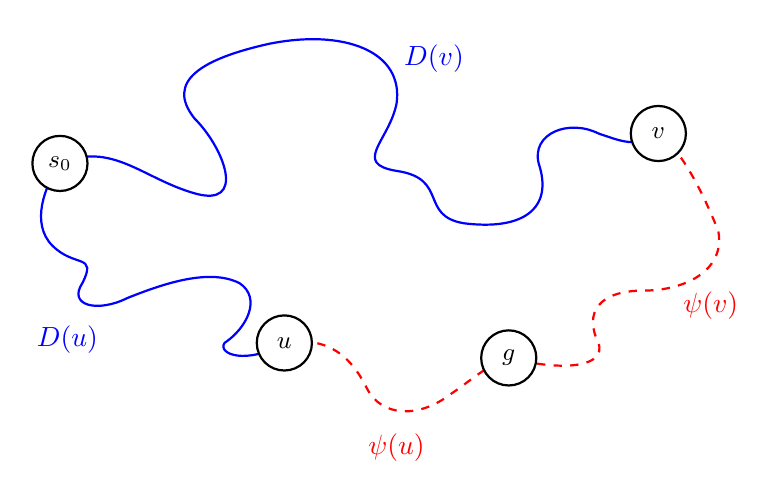
\begin{tikzpicture}[scale=0.95]

    \tikzset{
        vertex/.style={
            draw,
            circle,
            thick,
            fill=white,
            minimum size=7mm,
            inner sep=0pt,
            font=\small
        }
    }

    % body
    \coordinate (s0) at (0.0, 1.6);
    \coordinate (u)  at (3.0,-0.8);
    \coordinate (g)  at (6.0,-1.0);
    \coordinate (v)  at (8.0, 2.0);

    % modrá křivka: D(u)
    \draw[blue, thick]
        (s0)
        .. controls (-0.2,1.3) and (-0.4,0.8) .. (-0.1,0.5)
        .. controls ( 0.2,0.2) and ( 0.5,0.4) .. ( 0.3,0.0)
        .. controls ( 0.1,-0.3) and ( 0.5,-0.4) .. ( 0.9,-0.2)
        .. controls ( 1.4, 0.0) and ( 2.0, 0.2) .. ( 2.4, 0.0)
        .. controls ( 2.7,-0.2) and ( 2.5,-0.6) .. ( 2.2,-0.8)
        .. controls ( 2.1,-0.95) and ( 2.5,-1.1) .. (u);

    % modrá křivka: D(v)
    \draw[blue, thick]
        (s0)
        .. controls (0.7,1.9) and (1.1,1.4) .. (1.8,1.2)
        .. controls (2.5,1.0) and (2.2,1.8) .. (1.8,2.2)
        .. controls (1.4,2.7) and (1.9,3.0) .. (2.8,3.2)
        .. controls (3.8,3.4) and (4.6,3.1) .. (4.5,2.4)
        .. controls (4.4,1.9) and (3.9,1.6) .. (4.5,1.5)
        .. controls (5.2,1.4) and (4.8,0.9) .. (5.4,0.8)
        .. controls (6.2,0.7) and (6.6,1.0) .. (6.4,1.6)
        .. controls (6.3,2.0) and (6.8,2.2) .. (7.2,2.0)
        .. controls (7.5,1.9) and (7.7,1.8) .. (v);

    % červená křivka: psi(u)
    \draw[red, dashed, thick]
        (u)
        .. controls (3.6,-0.7) and (3.9,-1.0) .. (4.1,-1.4)
        .. controls (4.3,-1.8) and (4.8,-1.8) .. (5.2,-1.5)
        .. controls (5.5,-1.3) and (5.7,-1.1) .. (g);

    % červená křivka: psi(v)
    \draw[red, dashed, thick]
        (v)
        .. controls (8.3,1.8) and (8.6,1.2) .. (8.8,0.7)
        .. controls (8.9,0.2) and (8.4,-0.1) .. (7.8,-0.1)
        .. controls (7.2,-0.1) and (7.0,-0.4) .. (7.2,-0.8)
        .. controls (7.3,-1.1) and (6.8,-1.2) .. (g);

    % vrcholy
    \node[vertex] at (s0) {$s_0$};
    \node[vertex] at (u) {$u$};
    \node[vertex] at (v) {$v$};
    \node[vertex] at (g) {$g$};

    % popisky křivek
    \node[blue] at (0.1,-0.75) {$D(u)$};
    \node[blue] at (5.0,3.0) {$D(v)$};
    \node[red]  at (4.5,-2.2) {$\textcolor{red}{\psi(u)}$};
    \node[red]  at (8.7,-0.3) {$\textcolor{red}{\psi(v)}$};

\end{tikzpicture}
    \caption{Znázornění heuristické funkce $\psi$.}
    \label{fig:astar_heuristika}
\end{figure}
Součtu $D(v)+\psi(v)$ budeme říkat \emph{$f$-skóre}\footnote{V~anglických textech se pro dosud nalezenou vzdálenost často používá označení $g$ a~pro heuristiku $h$,~tedy $f(v)=g(v)+h(v)$.},~značíme jej $f(v)$. V~každé iteraci vybereme otevřený vrchol s~nejnižším $f$-skóre.

Ne každá heuristika zachová správnost této strategie. Budeme požadovat
\[\psi(g)=0\qquad\text{a}\qquad
\psi(u)\leqslant w(u,v)+\psi(v)\]
pro každou orientovanou hranu $(u,v)\in E$. Takové heuristice říkáme \emph{konzistentní}. Druhá podmínka je obdobou trojúhelníkové nerovnosti: odhad z~$u$ nesmí být větší než cena jednoho kroku do $v$ a~odhad z~$v$. Opakovaným použitím podél libovolné cesty z~$u$ do cíle dostaneme,~že $\psi(u)$ nikdy nepřeceňuje skutečnou nejkratší vzdálenost do cíle.

Oproti Dijkstrovu algoritmu tedy nenastává mnoho změn,~jen si navíc uchováváme hodnoty $f$-skóre.
\begin{algorithm}\label{alg:astar}
    \caption{\Astar}
    \KwIn{Nezáporně ohodnocený graf $G=(V,E,w)$,~vrcholy $v_0,g\in V$ a~konzistentní heuristika $\psi$}
    \tcp{Inicializace}
    \ForEach{\textup{vrchol $v\in V$}}{
        $stav(v)\gets$ \textit{nenalezený}\\
        $D(v)\gets\infty,\,f(v)\gets\infty$
    }
    $stav(v_0)\gets$ \textit{otevřený}\\
    $D(v_0)\gets 0,\,f(v_0)\gets\psi(v_0)$\\
    \While{\textup{existují otevřené vrcholy}}{
        $v\gets$ otevřený vrchol s~nejmenším $f$-skóre\\
        \If{$v=g$}{
            \Return{$D(g)$}
        }
        \ForEach{\textup{soused $s$ vrcholu $v$}}{
            \tcp{Našli jsme lepší cestu}
            \If{$stav(s)\neq\textit{uzavřený}$ a~$D(v)+w(v,s)<D(s)$}{
                $D(s)\gets D(v)+w(v,s)$\\
                $f(s)\gets D(v)+w(v,s)+\psi(s)$\\
                $stav(s)\gets$ \textit{otevřený}
            }
        }
        $stav(v)\gets$ \textit{uzavřený}
    }
    \Return{$\infty$}\\
    \KwOut{Vzdálenost $v_0$ od $g$}
\end{algorithm}

\subsection{Správnost algoritmu \Astar}

Podobně jako u~Dijkstrova algoritmu platí,~že při výběru vrcholu $v$ odpovídá $D(v)$ délce nejkratší cesty z~$v_0$ do $v$. Důkaz provedeme indukcí podle pořadí uzavíraných vrcholů.

Předpokládejme pro spor,~že vybíráme první vrchol $v$,~pro který je $D(v)>d(v_0,v)$. Na jedné nejkratší cestě do $v$ vezměme první dosud neuzavřený vrchol $x$ a~jeho již uzavřeného předchůdce $y$. Podle indukčního předpokladu bylo $D(y)=d(v_0,y)$,~takže po zpracování hrany $(y,x)$ platí $D(x)=d(v_0,x)$.
\begin{figure}[h]
    \centering
    \begin{tikzpicture}[scale=0.7, line cap=round, line join=round]
    % vertices
    \node[vertex] at (0.6,5.0)   (g)  {$g$};
    \node[vertex] at (-0.7,1.55) (v)  {$v$};
    \node[vertex] at (3.2,2.25)  (u)  {$v^{\prime}$};
    \node[vertex] at (3.2,-1.35) (s0) {$v_0$};

    % black curves D(v), D(u)
    \draw
        (v) .. controls (-0.35,1.15) and (-0.95,0.35) .. (-0.15,0.55)
            .. controls (0.45,0.75) and (0.25,1.65) .. (0.85,1.65)
            .. controls (1.30,1.45) and (0.95,-0.05) .. (1.55,-0.60)
            .. controls (2.05,-1.05) and (2.65,-0.85) .. (s0);
    \node at (0.45,-0.35) {$D(v)$};

    \draw
        (u) .. controls (2.65,1.95) and (2.75,1.45) .. (3.10,1.20)
            .. controls (3.55,0.90) and (3.55,0.35) .. (3.05,0.10)
            .. controls (2.70,-0.05) and (2.85,-0.25) .. (s0);
    \node[right=0.35cm] at (0.78,1.20) {$D(v^{\prime})$};

    % red edge from u to v
    \draw[edge, red!70!black]
        (u) .. controls (2.25,2.05) and (1.15,1.80) .. (v);
    \node[red!70!black, above] at (1.35,2.00) {$w(v,v^{\prime})$};

    % red dashed psi(v) -- corrected to end in g
    \draw[edge, red!70!black, dashed]
        (v) .. controls (-1.35,2.20) and (-0.95,3.35) .. (-0.20,3.10)
            .. controls (0.20,2.95) and (0.30,3.35) .. (0.05,3.60)
            .. controls (-0.20,3.85) and (0.00,4.10) .. (g);
    \node[red!70!black, left=2pt] at (-0.75,3.05) {$\psi(v)$};

    % blue dashed psi(u)
    \draw[blue!70!black, dashed]
        (g) .. controls (0.95,3.45) and (1.55,3.10) .. (2.20,3.30)
            .. controls (2.65,3.45) and (2.95,3.75) .. (3.05,3.75)
            .. controls (2.80,3.25) and (2.30,2.75) .. (1.95,2.45)
            .. controls (2.30,2.65) and (2.75,2.95) .. (3.05,3.00)
            .. controls (3.45,3.05) and (3.50,2.65) .. (3.15,2.35);
    \node[blue!70!black, above] at (2.55,3.55) {$\psi(v^{\prime})$};

\end{tikzpicture}
    \caption{Situace při výběru vrcholu $v$ při heuristice $\psi$,~kdy $D(v)$ neodpovídá délce nejkratší cesty.}
    \label{fig:astar_kratsi_cesta}
\end{figure}
Konzistenci můžeme opakovaně použít na část této cesty od $x$ do $v$. Dostaneme
\[\psi(x)\leqslant d(v_0,v)-d(v_0,x)+\psi(v).\]
Proto
\[
f(x)=D(x)+\psi(x)
\leqslant d(v_0,x)+d(v_0,v)-d(v_0,x)+\psi(v)
=d(v_0,v)+\psi(v)
<D(v)+\psi(v)=f(v).
\]
Vrchol $x$ je otevřený a~má menší $f$-skóre než $v$,~takže algoritmus měl vybrat $x$. To je spor. Každý uzavřený vrchol tedy dostane správnou vzdálenost; zvlášť to platí pro cílový vrchol $g$.

\warningbox{Konzistence heuristiky je pro uvedenou variantu algoritmu důležitá. Pokud by odhad tuto podmínku porušoval a~algoritmus uzavřené vrcholy znovu neotevíral,~mohl by některý vrchol uzavřít předčasně a~vrátit neoptimální cestu.}

\begin{remark}
    \begin{itemize}
        \item Dijkstrův algoritmus je speciálním případem \Astar. Stačí pro všechny vrcholy $v$ položit $\psi(v)=0$.
        \item Heuristiku bychom měli být schopni pro každý vrchol spočítat rychle. Ideální je konstantní čas $\bigO(1)$.
    \end{itemize}
\end{remark}

V~nejhorším případě může \Astar{} prozkoumat celý graf,~takže při použití binární haldy má stejný asymptotický horní odhad jako Dijkstrův algoritmus,~tedy $\bigO((n+m)\log n)$. Dobrá heuristika však obvykle výrazně sníží počet skutečně zpracovaných vrcholů. Volba $\psi=0$ neposkytne žádné směrování a~dostaneme přesně Dijkstrův algoritmus.

\subsection{Ukázky heuristických funkcí}

Zbývá zodpovědět otázku,~jakou heuristiku použít. Odpověď záleží na konkrétní úloze. Vraťme se k~bludišti,~v~němž se hráč pohybuje vodorovně nebo svisle o~jedno pole. Políčka identifikujeme souřadnicemi $(x,y)$.

Jednou možností je tzv. \emph{eukleidovská vzdálenost}. Ta je pro libovolnou dvojici bodů v~rovině $X=(x_1,y_1)$ a~$Y=(x_2,y_2)$ definována jako
\[\sqrt{(x_1-x_2)^2+(y_1-y_2)^2}.\]
Známe-li souřadnice cílového políčka,~můžeme eukleidovskou vzdálenost použít jako heuristiku $\psi_E$. Překážky ignorujeme,~takže dostaneme dolní odhad skutečné délky cesty. Situaci lze sledovat na obrázku \ref{fig:astar_bludiste_euclid}.
\begin{figure}[h]
    \centering
    \input{01-grafalgo/images/ch01_astar_mrizka_euclid.tex}
    \caption{Příklad bludiště s~eukleidovskou heuristikou.}
    \label{fig:astar_bludiste_euclid}
\end{figure}
Protože se v~našem bludišti nelze pohybovat po diagonálách,~ještě přirozenější volbou je \emph{manhattanská vzdálenost} $\psi_M$ definovaná vztahem
\[\abs{x_1-x_2}+\abs{y_1-y_2}.\]
\begin{figure}[h]
    \centering
    \input{01-grafalgo/images/ch01_astar_mrizka_manhattan.tex}
    \caption{Příklad bludiště s~manhattanskou heuristikou.}
    \label{fig:astar_bludiste_manhattan}
\end{figure}
Eukleidovská i~manhattanská vzdálenost splňují trojúhelníkovou nerovnost,~a~proto v~této mřížce dávají konzistentní heuristiky. Manhattanská vzdálenost je zde navíc přesnější: bez překážek se rovná skutečnému počtu vodorovných a~svislých kroků do cíle. Její větší hodnota tedy není nevýhodou,~dokud nepřeceňuje skutečnou cenu cesty. Naopak zpravidla lépe směruje hledání.
